\chapter{Diseño e implementación}

\label{Chapter3}

En el presente capítulo se presentan los detalles del diseño y los criterios adoptados para el desarrollo del trabajo junto con los pasos seguidos para su implementación.

\section{Arquitectura del sistema}

El sistema tiene una configuración de arquitectura del tipo cliente-servidor. Está constituido por dos nodos y un servidor, los cuales están conectados a la red local y se comunican a través del protocolo MQTT. El servidor recibe los parámetros actuales de estado y cambios desde cada dispositivo, los procesa y almacena en la base de datos. También envía mensajes hacia los dispositivos para cambiar el estado de las salidas o el parámetro que se desee cambiar. Los usuarios pueden consultar y modificar el estado de los dispositivos desde un navegador web móvil o desde una computadora.

En la figura \ref{fig:9} se puede observar la arquitectura cliente-servidor del sistema implementado en el trabajo.

\begin{figure}[h]
\centering
\includegraphics[scale=0.4]{Imagen 9 - cliente-servidor.jpg}
\caption[Arquitectura cliente-servidor]{Arquitectura cliente-servidor. \footnotemark}
\label{fig:9}
\end{figure}
\footnotetext{Imagen tomada de: \url{https://www.bujarra.com/raspberry-pi-servidor-vpn-con-pptp/}}

Uno de los nodos tiene como función sensar y controlar de temperatura de un recinto, y el otro controlar la iluminación. Originalmente el proyecto estaba pensado para que un solo nodo implemente estas dos funciones, pero durante el desarrollo se optó por la implementación separada. Este cambio se basó en la idea de modularizar los nodos y que sus funciones sean específicas. De esta forma es más amigable para el usuario visualizar y modificar el estado en pantalla e implementar el alta de nuevos dispositivos en el sistema.

El servidor está montado sobre una Raspberry Pi 400 con un sistema operativo Raspbian con interfaz gráfica. Este sistema operativo es la versión oficial ofrecida por la fundación Rasperry Pi y está basado en Debian versión 11 (\textit{bullseye}). En esta etapa de desarrollo se optó por una Raspberry Pi 400 por una cuestión de costos y practicidad a la hora de desarrollar y hacer las pruebas, aunque tiene un mayor volumen que los otros modelos de la familia. Al momento de ofrecer una solución definitiva está pensado que sea implementado en una placa con el formato más pequeño como cualquiera de las Raspberry Pi 4. La conexión del servidor a la red local es por cable Ethernet.

\subsection{Especificaciones técnicas del servidor}

El sistema operativo del servidor está instalado y se ejecuta desde un disco de estado sólido por USB. Este tipo de discos tienen una mayor capacidad de escrituras y lecturas que una memoria microSD, lo que resulta favorable al momento de hacer modificaciones y pruebas de ejecución de software. En la versión final del sistema todo el software estará instalado en una tarjeta microSD para que todo el conjunto sea lo más pequeño posible.

En la tabla \ref{tab:Especificaciones Raspberry Pi 400} pueden verse las especificaciones técnicas de hardware más importantes del modelo Raspberry Pi 400.

\begin{table}[h]
\centering
\caption[Raspberry Pi 400]{Especificaciones de Raspberry Pi 400.}
\begin{tabular}{l c}
\toprule
Procesador		&	Broadcom BCM2711 quad-core Cortex-A72(ARM v8) \\
				&	64-bit SoC @ 1.8GHz \\
\midrule
Memoria			&	4GB LPDDR4-3200 \\
\midrule
				&	2.4GHz and 5.0GHz 802.11b/g/n/ac wireless LAN \\
Conectividad		&	Bluetooth 5.0, BLE\\
				&   Gigabit Ethernet \\
\midrule
Alimentación		&	5V DC vía USB-C\\
\bottomrule
\hline
\end{tabular}
\label{tab:Especificaciones Raspberry Pi 400}
\end{table}

\section{Modelo de datos}

En esta sección se describen las diferentes tablas dentro de la base de datos de tipo relacional MariaDB llamada \textit{Domotica}. Con el objetivo de mostrar una representación visual fácil de comprender se muestran las imágenes representadas en la página phpMyadmin. Las tablas que forman dicha base son:

\begin{itemize}
	\item Dispositivos.
	\item Usuarios.
	\item Mediciones.
\end{itemize}

Debe tenerse en cuenta que todo el contenido que se ejecuta del lado del servidor se encuentra dentro de un contenedor Docker. Dicho contenido corresponde a las imágenes de los servicios de Ionic, MariaDB, phpMyAdmin, backend con Node y mosquitto. En la figura \ref{fig:10} se observa el contenido del archivo \textit{docker-compose.yml} pertinente a la configuración de los servicios de MariaDB y phpMyAdmin.

\begin{figure}[h]
\centering
\includegraphics[scale=0.6]{Imagen 10 - Docker base datos.jpg}
\caption[Docker base datos]{Configuración de Docker de la base de datos. \footnotemark}
\label{fig:10}
\end{figure}

\subsection{Tabla Dispositivos}

Esta tabla contiene los datos de los dispositivos dados de alta en el sistema. Dichos datos son el ID del dispositivo, el nombre, la ubicación, la dirección MAC, el tipo, el valor de la alarma y el estado de la alarma (0 para desactivada y 1 para activada).

En la figura \ref{fig:11} puede verse la tabla cargada con 2 dispositivos funcionando.

\begin{figure}[h]
\centering
\includegraphics[scale=0.6]{Imagen 11 - Tabla dispositivos.jpg}
\caption[Tabla dispositivos]{Tabla de dispositivos. \footnotemark}
\label{fig:11}
\end{figure}

El ID del dispositivo es un número brindado por el fabricante del dispositivo que consta de 13 números y está formado por: los primeros 2 dígitos que corresponden al tipo de dispositivo (el sistema está pensado para cubrir hasta un total de 100 tipos de dispositivos, aunque en esta etapa de prototipo sólo se hayan desarrollado 2); 4 dígitos de seguridad fijos que en este caso son "2819" y sirven para corroboración y como seguridad; y los últimos 5 dígitos corresponden al número de serie del equipo (2 para el año, 2 para la semana y 3 para el número de fabricación del equipo en esa semana, en ese orden). Como puede observarse, el sistema está pensado para que en un futuro sea parte de una producción en serie.

Tanto el nombre como la ubicación son campos alfanuméricos elegidos por el usuario para describir al dispositivo. La dirección MAC es enviada por el dispositivo la primera vez que se conecta al sistema y no se completa por el usuario. El tipo corresponde al tipo de sensor y para esta etapa del desarrollo puede ser "Temperatura" o "Luz dimmer".

El valor de la alarma es un campo numérico y sólo tiene efecto para dispositivos del tipo de temperatura. Se enviará una notificación por mail cada vez que el valor enviado por el dispositivo sea mayor o igual al seteado en este campo, siempre que dicha alarma esté activada en el campo.

\subsection{Tabla Usuarios}

La tabla de usuarios contiene todos los datos relacionados a aquellas personas que vayan a utilizar el sistema. En esta etapa está implementado con 3 usuarios, ya que al ser de tipo hogareño resultaría difícil que más de 3 personar dentro de una misma casa se registren. Pero con pocos cambios el sistema podría ser escalable a la cantidad de usuarios que se desee, generando una página de alta de usuarios.

Los valores almacenados en esta tabla son el ID de usuario (de 1 a 3), el nombre de usuario, la clave, el nombre de la persona y su apellido, su e-mail y un campo de tipo booleano que se modificará cuando se haya actualizado por primera vez. Cabe aclarar que cada vez que se ingrese al sistema con un usuario que no haya actualizado sus datos, se mostrará en pantalla un aviso para que este actualice sus datos.

En la figura \ref{fig:12} puede verse la tabla cargada con los 3 usuarios de los cuales hay 2 actualizados y el tercero tiene los valores por defecto.

\begin{figure}[h]
\centering
\includegraphics[scale=0.6]{Imagen 12 - Tabla usuarios.jpg}
\caption[Tabla usuarios]{Tabla de usuarios. \footnotemark}
\label{fig:12}
\end{figure}

\subsection{Tabla Mediciones}

La tabla de mediciones contiene todos los datos referentes a las mediciones realizadas por los dispositivos y los datos de modo seleccionado. Los dispositivos reportan cada 5 minutos estos datos y se almacenan en esta tabla.

Los datos almacenados en esta tabla son: el ID de la medición (un valor autoincremental), el ID del dispositivo, el tipo de dispositivo, la fecha y hora de la medición, el valor de la medición, el modo de funcionamiento (manual o automático), el valor de la salida (si es de tipo temperatura es 0 o 100 y corresponde a encendido o apagado, y si es de tipo luz dimmer va de 0 a 100 con saltos de 10), y la hora y minutos de encendido y apagado para el modo automático.

En la figura \ref{fig:13} pueden verse algunas de las mediciones dentro de la correspondiente tabla, ordenadas por ID. Cabe aclarar que sólo se ven algunas ya que los dispositivos se encuentran reportando y llenando de datos la base.

\begin{figure}[h]
\centering
\includegraphics[scale=0.6]{Imagen 13 - Tabla mediciones.jpg}
\caption[Tabla mediciones]{Tabla de mediciones. \footnotemark}
\label{fig:13}
\end{figure}

\section{Desarrollo del frontend}

El frontend del presente trabajo fue desarrollado en el lenguaje TypeScript con Angular como \textit{framework} integrado con Ionic. El prototipo de aplicación está diseñado para acceder desde un navegador web tanto desde una computadora como un móvil, pero se optó por usar Ionic para un posterior desarrollo de una aplicación para sistemas operativos móviles. Es por esto que en esta instancia puede referirse a la aplicación web como una SPA y no como una PWA.

En la figura \ref{fig:14} se puede observar el fragmento de código correspondiente a la configuración de Ionic dentro del archivo \textit{docker-compose.yml}.

\begin{figure}[h]
\centering
\includegraphics[scale=0.6]{Imagen 14 - Docker ionic.jpg}
\caption[Configuración Ionic]{Configuración de Docker de Ionic. \footnotemark}
\label{fig:14}
\end{figure}

La estructura de archivos de cada página esta diseñada de la misma forma como se muestra en la imagen \ref{fig:15}. Allí se pueden ver como ejemplo los archivos que componen la página \textit{home}.

\begin{figure}[h]
\centering
\includegraphics[scale=0.6]{Imagen 15 - Estructura.jpg}
\caption[Estructura página]{Estructura de archivos de página. \footnotemark}
\label{fig:15}
\end{figure}

Además se utilizaron interfaces para definir las estructuras de datos de los dispositivos, las mediciones y los usuarios, y servicios para el proceso de autenticación y de consultas HTTP al backend, que serán explicadas posteriormente.

El servicio de autenticación consta de el ingreso de un usuario y contraseña en la página de \textit{login} que se comparan con los que están almacenados en la base de datos. Si dichos valores ingresados corresponden con alguno de los existentes, se genera un \textit{token} desde el backend que se almacena en el dispositivo que está haciendo la consulta. Esto permite que se puedan acceder a las demás páginas de la aplicación.

En el código \ref{lst:Autenticación de rutas} puede verse el fragmento de la autenticación del archivo \textit{auth.guard.ts}

\definecolor{dkgreen}{rgb}{0,0.6,0}
\definecolor{gray}{rgb}{0.5,0.5,0.5}
\definecolor{mauve}{rgb}{0.58,0,0.82}

\lstset{frame=tb,
  language=Java,
  aboveskip=3mm,
  belowskip=3mm,
  captionpos=b,
  showstringspaces=false,
  columns=flexible,
  basicstyle={\small\ttfamily},
  numbers=left,
  numberstyle=\tiny\color{gray},
  keywordstyle=\color{blue},
  commentstyle=\color{dkgreen},
  stringstyle=\color{mauve},
  breaklines=true,
  breakatwhitespace=true,
  tabsize=3,
}

\begin{lstlisting}[caption={Autenticación de rutas}, label={lst:Autenticación de rutas}]
export class AuthGuard {
  constructor(private _loginService: LoginService, private _router: Router) {}
  canActivate(
    route: ActivatedRouteSnapshot,
    state: RouterStateSnapshot): Observable<boolean | UrlTree> | Promise<boolean | UrlTree> | boolean | UrlTree {
    if (!this._loginService.logIn) {
      this._router.navigate(['/login'])
      return false
    }
    return true;
  }
}
\end{lstlisting}

El \textit{route guard} es una característica del Angular Router que permite ejecutar algún tipo de lógica cuando se solicita una ruta, y basado en esa lógica, se permite o denega el acceso al usuario a esa ruta. Comúnmente es utilizado para verificar si un usuario está logueado o no en el sistema para verificar si tiene autorización para acceder a esa URL.

El \textit{route guard} se puede agregar implementando la interfaz \textit{CanActivate} disponible en \textit{@angular/router} y allí implementar el método \textit{canActivate()} que contendrá la lógica para denegar o permitir el acceso a la ruta.\citep{22}

En todas las páginas de la aplicación se utilizan los métodos \textit{ngOnInit} y \textit{ngOnDestroy}. Ambos son métodos de Angular en el ciclo de vida de un componente. Sus funciones son la inicialización de variables y configuración de un componente y la liberación de recursos antes que el componente se destruya.\citep{23}

\subsection{Rutas y páginas destacadas}

Las rutas disponibles en la aplicación se describen en la tabla \ref{tab:rutas}. A través de ellas se navega dentro de la aplicación y se accede a las distintas pantallas. Estas rutas se encuentran definidas en el archivo \textit{app-routing.module.ts} donde además se hace referencia al módulo de la aplicación que debe abrirse al acceder a cada una de las rutas listadas.

\begin{table}[h]
\centering
\caption[Rutas]{Rutas de la aplicación}
\begin{tabular}{l l}
\toprule
\textbf{Ruta} 			& \textbf{Descripción}\\
\midrule
/login					& Pantalla de inicio de sesión\\
/home					& Pantalla principal con funciones y listado de dispositivos\\
/usuario/:userId			& Pantalla de edición de datos de usuario\\
/ayuda					& Pantalla de manual de usuario\\
/dispositivos/:id		& Pantalla de visualización de estado del dispositivo\\
/medicion/:id			& Pantalla de visualización de las mediciones del\\
/grafico/:id				& Pantalla de visualización del gráfico de las mediciones\\
/config/:id				& Pantalla de configuración del dispositivo\\
/modificar/:id			& Pantalla de edición de datos de un dispositivo existente\\
/agregar					& Pantalla para agregar un dispositivo nuevo\\
\bottomrule
\hline
\end{tabular}
\label{tab:rutas}
\end{table}

En los casos en los que se encuentra el campo \textit{:id}, este valor se completa con el valor de identificador del elemento en cuestión. En el caso de los usuarios, cada uno de ellos tiene un identificador, lo mismo que para los dispositivos. Para las rutas \textit{medicion}, \textit{grafico}, \textit{config} y \textit{modificar} el \textit{:id} al que se hace referencia es el del dispositivo al que se quiere leer o modificar.

\subsubsection{Pantalla de \textit{login}}

En la figura \ref{fig:16} se muestra la página de inicio de sesión en la aplicación.

\begin{figure}[h]
\centering
\includegraphics[scale=0.38]{Imagen 16 - Login.png}
\caption[Pantalla login]{Pantalla de \textit{login}. \footnotemark}
\label{fig:16}
\end{figure}

El sistema trae la posibilidad de configurar 3 usuarios distintos para que utilicen, visualicen y configuren la aplicación. Todos poseen el mismo rol y pueden configurar cualquier campo que corresponda a dicho usuario ingresando en la opción Usuario dentro de la pantalla principal.

\subsubsection{Pantalla principal \textit{home}}

En la figura \ref{fig:17} puede verse la pantalla principal de la aplicación. En la parte superior se encuentran los botones principales de la aplicación tales como el de configuración del usuario actual, cerrar sesión y la página de ayuda o manual de usuario. En la parte inferior se encuentra el listado de dispositivos implementado con \textit{ion-cards} los cuales permiten ver el estado de cada dispositivo, modificar los datos y alarma del dispositivo y eliminarlo de la lista. Hay que tener en cuenta que al borrar un dispositivo del sistema se borran también todas las mediciones y documentos asociados a él dentro de la base de datos.

\begin{figure}[h]
\centering
\includegraphics[scale=0.38]{Imagen 17 - Home.png}
\caption[Pantalla home]{Pantalla de \textit{home}. \footnotemark}
\label{fig:17}
\end{figure}

Por último en la parte inferior de la pantalla principal se encuentra el botón para agregar un dispositivo nuevo. Dicho botón dirige a la página de creación de un dispositivo nuevo.

\subsubsection{Pantalla de creación de dispositivo nuevo}

En la pantalla que se muestra en la figura \ref{fig:18} se deben cargar los datos de un dispositivo nuevo. Esto es importante ya que aquí se dan de alta los dispositivos nuevos que se incorporar al sistema.

\begin{figure}[h]
\centering
\includegraphics[scale=0.45]{Imagen 18 - Agregar.png}
\caption[Pantalla home]{Pantalla de creación de dispositivo nuevo. \footnotemark}
\label{fig:18}
\end{figure}

Aquí deben colocarse los datos de ubicación del nodo, el nombre con el que se desea identificarlo, el ID de fabricante, el tipo, y los valores de la alarma en caso de que se trate de un nodo de temperatura. El estado de la alarma puede configurarse pro primera vez en esta sección, pero puede modificarse cuando se desee. Se debe tener en cuenta que al momento existen 2 tipos de dispositivos: temperatura y luz dimmer. Solo se encuentra habilitada la alarma para los nodos del tipo de temperatura ya que no tiene sentido colocar una alarma a un nodo que no realiza mediciones ni controla parámetros críticos.

El ID del fabricante es un número de 13 dígitos compuesto de la siguiente forma: los 2 primeros identifican el tipo de dispositivo; los 4 que le siguen son obligatoriamente los números "2819", y se colocan como número de identificación del sistema y como seguridad; los 2 dígitos que le siguen son el año de fabricación del dispositivo; los 2 que le siguen son la semana de fabricación; y por último los 3 dígitos que restan son el número de fabricación en esa semana, es decir que comienza en el "000" y termina en "999". Este número resultante será entregado por el fabricante y será único para cada dispositivo.

Desde el frontend se verifica que se ingrese el código de seguridad dentro del ID del fabricante en el fragmento de código \ref{lst:Verificación de ID}:

\begin{lstlisting}[caption={Verificación de ID}, label={lst:Verificación de ID}]
verificarID(dispositivoId: string): boolean {
    const posicion = 2;
    return dispositivoId.charAt(posicion) === '2' &&
      dispositivoId.charAt(posicion + 1) === '8' &&
      dispositivoId.charAt(posicion + 2) === '1' &&
      dispositivoId.charAt(posicion + 3) === '9';
  }
\end{lstlisting}

Una vez que el dispositivo nuevo esté dado de alta, al encenderlo se va a conectar a la red y va a registrar automáticamente la dirección MAC dejándola guardada en la tabla de dispositivos.

\subsubsection{Pantalla de configuración de modo}

En esta sección se va a configurar el modo de trabajo y todos los parámetros asociados. En la figura \ref{fig:19} puede observarse la pantalla típica de configuración de un dispositivo de temperatura.

\begin{figure}[h]
\centering
\includegraphics[scale=0.45]{Imagen 19 - Enviar datos.png}
\caption[Pantalla de configuración de modo]{Pantalla de configuración de modo. \footnotemark}
\label{fig:19}
\end{figure}

En la parte superior se puede elegir el estado de la salida en modo manual si fuese un dispositivo de temperatura y el valor de la salida de 0 a 100 si fuese un dimmer. Luego sigue la configuración del modo automático con el set point y las horas de encendido y apagado. Por último en la parte inferior se puede elegir el modo, automático o manual.

Al cargarse la página de configuración se leen los datos de la última medición del dispositivo y se autocompletan las variables de configuración con estos valores por defecto. Una vez que se hayan seleccionado todos los valores, se debe hacer clic en enviar para que se envíen los datos al dispositivo.

\subsubsection{Pantallas de mediciones y gráfico}

En la figura \ref{fig:20} puede verse el gráfico de medición actual de temperatura del correspondiente nodo.

\begin{figure}[h]
\centering
\includegraphics[scale=0.55]{Imagen 20 - Grafico temperatura.png}
\caption[Pantalla de configuración de modo]{Pantalla de configuración de modo. \footnotemark}
\label{fig:20}
\end{figure}

Se utiliza un gráfico de la biblioteca online \textit{highcharts} y se importa desde el archivo \textit{dispositivo.page.ts} como se muestra en el fragmento de código \ref{lst:highcharts}. Esta biblioteca posee varios modelos para desarrollo web y móvil para frameworks tales como Javascript, Angular, React, VueJS, iOS, R, .NET, Python y más\citep{24}.

\begin{lstlisting}[caption={Importación de gráfico de \textit{highcharts}}, label={lst:highcharts}]
import * as Highcharts from 'highcharts';
\end{lstlisting}

En la figura \ref{fig:21} pueden verse las mediciones del dispositivo de temperatura ordenadas desde la más nueva a la más antigua.

\begin{figure}[h]
\centering
\includegraphics[scale=0.38]{Imagen 21 - Mediciones.png}
\caption[Pantalla de mediciones del ddispositivo de temperatura]{Pantalla de mediciones del ddispositivo de temperatura. \footnotemark}
\label{fig:21}
\end{figure}

En caso que se squieran borrar se puede hacer con el botón correspondiente como se muestra en la parte superior de la misma figura. Esta opcioón se agegó en caso de que el usuario no desee ver las mediciones antiguas.

Además se puede acceder a una página que muestre una representación gráfica de las mediciones del día en curso. Esto hace que sea más fácil leer las mediciones y poder sacar conclusiones o datos que se necesiten. En la figura \ref{fig:22} puede verse un ejemplo de gráfico de mediciones reales tomadas por el sensor de temperatura y alamcenadas en la base de datos. Se utilizó un gráfico de \textit{highcharts} también cuya función es hacer gráficos temporales basados en mediciones.

\begin{figure}[h]
\centering
\includegraphics[scale=0.38]{Imagen 22 - Grafico.png}
\caption[Pantalla de presentación gráfica de mediciones]{Pantalla de presentación gráfica de mediciones. \footnotemark}
\label{fig:22}
\end{figure}

\section{Desarrollo del backend}

El backend fue desarrollado en Node.js mediante JavaScript y Express. Posee un archivo principal \textit{index.js} del cual se llaman los distintos archivos que tengan funciones, \textit{endpoints} e inicializaciones de otros módulos y que tengan relación con el backend. Con lo anterior se realizó una primera versión de modularización del código del backend.

En el código \ref{lst:Configuracion de index.js}:

\begin{lstlisting}[caption={Configuración de \textit{index.js}}, label={lst:Configuracion de index.js}]
const express = require('express');
const app = express();
const pool = require('./mysql-connector');
const cors = require('cors');
const jwt = require('jsonwebtoken');
const mqtt = require('mqtt');
const fs = require('fs');
const mqttClient = require('./mqtt-handler');
const transporter = require('./nodemailer');
const { authRouter } = require('./auth');
const { JWT_Secret } = require('./auth');
const { dispositivosRouter, ultMedicionRouter, graficoRouter, medicionesRouter, deleteDispositivoRouter, estadoConexionRouter, borrarTablaRouter, usuariosRouter, agregaRouter, modificarDispositivoRouter } = require('./dispositivos');
\end{lstlisting}

Aquí se puede ver que se inicializa Express, la base de datos, \textit{cors} para poder conectarse a la API, \textit{jsonwebtoken} para la generación del token, \textit{mqtt} y su configuración, el gestor de mail \textit{nodemailer} para la generación de mails para las alarmas y el archivo \textit{dispositivos.js} con las funciones que se reciben en cada endpoint.

\subsection{Conexión a la base de datos}

La conexión con la base de datos se realiza en el archivo \textit{mysql-connector.js} y se muestra en el código \ref{lst:Conexion de base}.

\begin{lstlisting}[caption={Conexión con la base de datos}, label={lst:Conexion de base}]
const configmariadb = {
  connectionLimit: 20,
  host: '192.168.0.70',
  port: '3306',
  user: 'root',
  password: 'userpass',
  database: 'Domotica'
};

const pool = mariadb.createPool(configmariadb);

console.log("Iniciando DB");

(async () => {
  try {
    const connection = await pool.getConnection();
    console.log ("Conexion exitosa a", configmariadb.database, "a", configmariadb.host, ":", configmariadb.port);
    connection.release();
  } catch (err) {
    console.log ("Error al establecer la conexion:", err);
    process.exit(1);
  }
})();

module.exports = pool;
\end{lstlisting}

En la primera sección del código se configura la conexión estableciendo la URL y puerto de conexión, así como también los datos para poder acceder y el nombre de la base. Luego se crea un pool de conexiones usando \textit{mariadb.createPool} con la configuración definida en configmariadb. Un \textit{pool} es una colección de conexiones reutilizables a la base de datos que se gestionan automáticamente para optimizar el rendimiento. Por último se utiliza una función asíncrona anónima para intentar establecer una conexión a la base de datos y emite mensajes por consola dependiendo si se conecta con éxito o tiene un error. Finalmente, el objeto \textit{pool} se exporta, lo que permite que otros módulos de la aplicación accedan al \textit{pool} de conexiones para interactuar con la base de datos.

\subsection{Configuración de la conexión \textit{mqtt}}

En el documento \textit{mqtt-handler.js} se encuentra la configuración del broker \textit{mosquitto} y de los \textit{topics} utilizados de \textit{mqtt}. En el código \ref{lst:Config mqtt} se muestra el fragmento de inicialización del broker.

\begin{lstlisting}[caption={Inicialización del broker \textit{mqtt}}, label={lst:Config mqtt}]
const caCert = fs.readFileSync('/home/node/app/certs/ca.pem');
const privateKey = fs.readFileSync('/home/node/app/certs/client.key');
const clientCert = fs.readFileSync('/home/node/app/certs/client.pem');
console.log('Certificados SSL para MQTT leidos correctamente');

const mqttBrokerUrl = '192.168.0.70';
const mqttOptions = {
  host: mqttBrokerUrl,
  port: 8883,
  protocol: 'mqtts',
  ca: caCert,
  key: privateKey,
  cert: clientCert,
};
\end{lstlisting}

Como se puede observar se leen los certificados TLS generados con anterioridad para añadir seguridad a la comunicación dentro del sistema utilizando \textit{OpenSSL}. Este es un software desarrollado por el Proyecto OpenSSL, y está compuesto por un conjunto de herramientas robusto, de calidad comercial y con todas las funciones para criptografía de uso general y comunicación segura.\citep{25}

\subsection{Configuración del envío de mails}

Para el envío de mails al dispararse una alarma se utilizó \textit{Nodemailer}, que es un módulo de \textit{Node.js} para permitir el envío de mails. Las principales características son: es un único módulo sin dependencias, gran enfoque en la seguridad, soporte \textit{Unicode} para usar cualquier carácter incluidos emojis y soporte de contenido HTML y texto sin formato, entre otras.\citep{26}

La configuración de el módulo de envío de mensajes se configura como se describe en el código \ref{lst:Nodemailer}. Además de este archivo, se debió configurar la cuenta de mail para que pueda aceptar conexiones desde otras aplicaciones en la configuración de seguridad de Google.

\begin{lstlisting}[caption={Configuración del módulo de envío de mails}, label={lst:Nodemailer}]
const nodemailer = require('nodemailer');

const transporter = nodemailer.createTransport({
    service: 'gmail',
    user: "smtp.gmail.com",
    port: 465,
    secure: true,
    auth: {
      type: 'login',
      user: 'automaticoh@gmail.com',
      pass: '**** **** **** ****'
    }
  });

module.exports = transporter;
\end{lstlisting}

\subsection{API y rutas}

Una interfaz de programación de aplicación o API (en inglés, \textit{Application Programming Interface}) es un conjunto de reglas y protocolos que permite que diferentes aplicaciones se comuniquen entre sí. En el contexto de la programación web, las APIs son comunes para permitir la interacción entre aplicaciones cliente y servicios web. En este caso está definida en el archivo \textit{dispositivos.js} y contiene las rutas, funciones y métodos HTTP recibidos en cada consulta desde el frontend, permitiendo interactuar con los otros componentes del sistema.

En el desarrollo del trabajo se utilizan los métodos get, put, post y delete en las distintas rutas. Por ejemplo, en el código \ref{lst:Consulta MariaDB} se puede ver el fragmento de backend que recibe la consulta de listado de dispositivos y hace la propia consulta a la base de datos.

\begin{lstlisting}[caption={Consulta de listado de dispositivos al backend}, label={lst:Consulta MariaDB}]
dispositivosRouter.get('/:id', async function (req, res, next) {
    try {
      const connection = await pool.getConnection();
      const result = await connection.query('SELECT * FROM Dispositivos WHERE dispositivoId = ?', req.params.id);
      connection.release();
      res.send(JSON.stringify(result)).status(200);
    } catch (err) {
      res.send(err).status(400);
    }
  });
\end{lstlisting}

Por último, en este archivo se exportan todas las rutas definidas para poder utilizarlas en cualquier módulo que se lo requiera.

\section{Nodos, sensores y actuadores}

En esta sección se describen las características más destacadas de los componentes de hardware del sistema. El software embebido de los microcontroladores se desarrolló con el \textit{framework} ESP-IDF \citep{27} en Visual Studio Code.

Para el proyecto se utilizaron fragmentos de código desarrollados en diversas materias del posgrado así como también librerías para este \textit{framework} disponibles en Github. Una de estas librerías corresponde al manejo del display con interfaz SSD1306 \citep{28}. Otro repositorio utilizado fue el que suministró el código para el manejo del sensor de temperatura DHT22 y el encoder rotativo con pulsador \citep{29}.

Dentro de la carpeta \textit{main} del software de los nodos se encuentran además los certificados SSL necesarios para que el dispositivo pueda comunicarse con el broker como se muestra en a figura \ref{fig:23}.

\begin{figure}[h]
\centering
\includegraphics[scale=0.9]{Imagen 23 - Certificados.png}
\caption[Certificados]{Ubicación de los certificados SSL.}
\label{fig:23}
\end{figure}

\subsection{Características de los nodos}

Los nodos están compuestos por el módulo central y los periféricos de entrada y salida, que son los sensores y los actuadores. En el desarrollo del trabajo se utilizó una versión de módulo central con un microcontrolador ESP32 incluido en una placa de desarrollo. En la tabla \ref{tab:esp32} pueden verse las características de hardware más importantes de este modelo de dispositivo.

\begin{table}[h]
\centering
\caption[Módulos ESP32]{Especificaciones técnicas del módulo ESP32 \citep{30}.}
\begin{tabular}{l c c}
\toprule
\textbf{Característica} & \textbf{ESP32}\\
\midrule
Núcleo			& Xtensa® dual-core 32-bit LX6\\
				& @240 MHz\\
Flash			& 0 MB, 2 MB o 4MB\\
				& (dependiendo la versión)\\
Protocolo Wi-Fi	& 802.11 b/g/n, 2.4 GHz\\
\bottomrule
\hline
\end{tabular}
\label{tab:esp32}
\end{table}

En la figura \ref{fig:24} puede observarse el diagrama en bloques del nodo de temperatura y control de calefacción. Los periféricos de entrada son el encoder y el sensor de temperatura y los de salida son el display que muestra la información y la salida de potencia.

\begin{figure}[h]
\centering
\includegraphics[scale=1.3]{Imagen 24 - Nodo temperatura.jpg}
\caption[Nodo de temperatura]{Diagrama en bloques del nodo de temperatura.}
\label{fig:24}
\end{figure}

En la figura \ref{fig:25} puede verse el diagrama en bloques del nodo de dimerización de la luminaria de corriente continua. En este caso, a diferencia del modelo descripto antes, posee un solo periférico de entrada y el de salida controla una salida de corriente continua de 5 a 24 V. En el caso del proyecto se utilizó una luminaria de 5 V y un consumo de 200 mA.

\begin{figure}[h]
\centering
\includegraphics[scale=1.3]{Imagen 25 - Nodo dimmer.jpg}
\caption[Nodo dimer]{Diagrama en bloques del nodo de dimerización.}
\label{fig:25}
\end{figure}

En la figura \ref{fig:26} se muestra la placa de desarrollo con el ESP32 montada sobre una placa adicional para facilitar las conexiones y la alimentación de los periféricos. 

\begin{figure}[h]
\centering
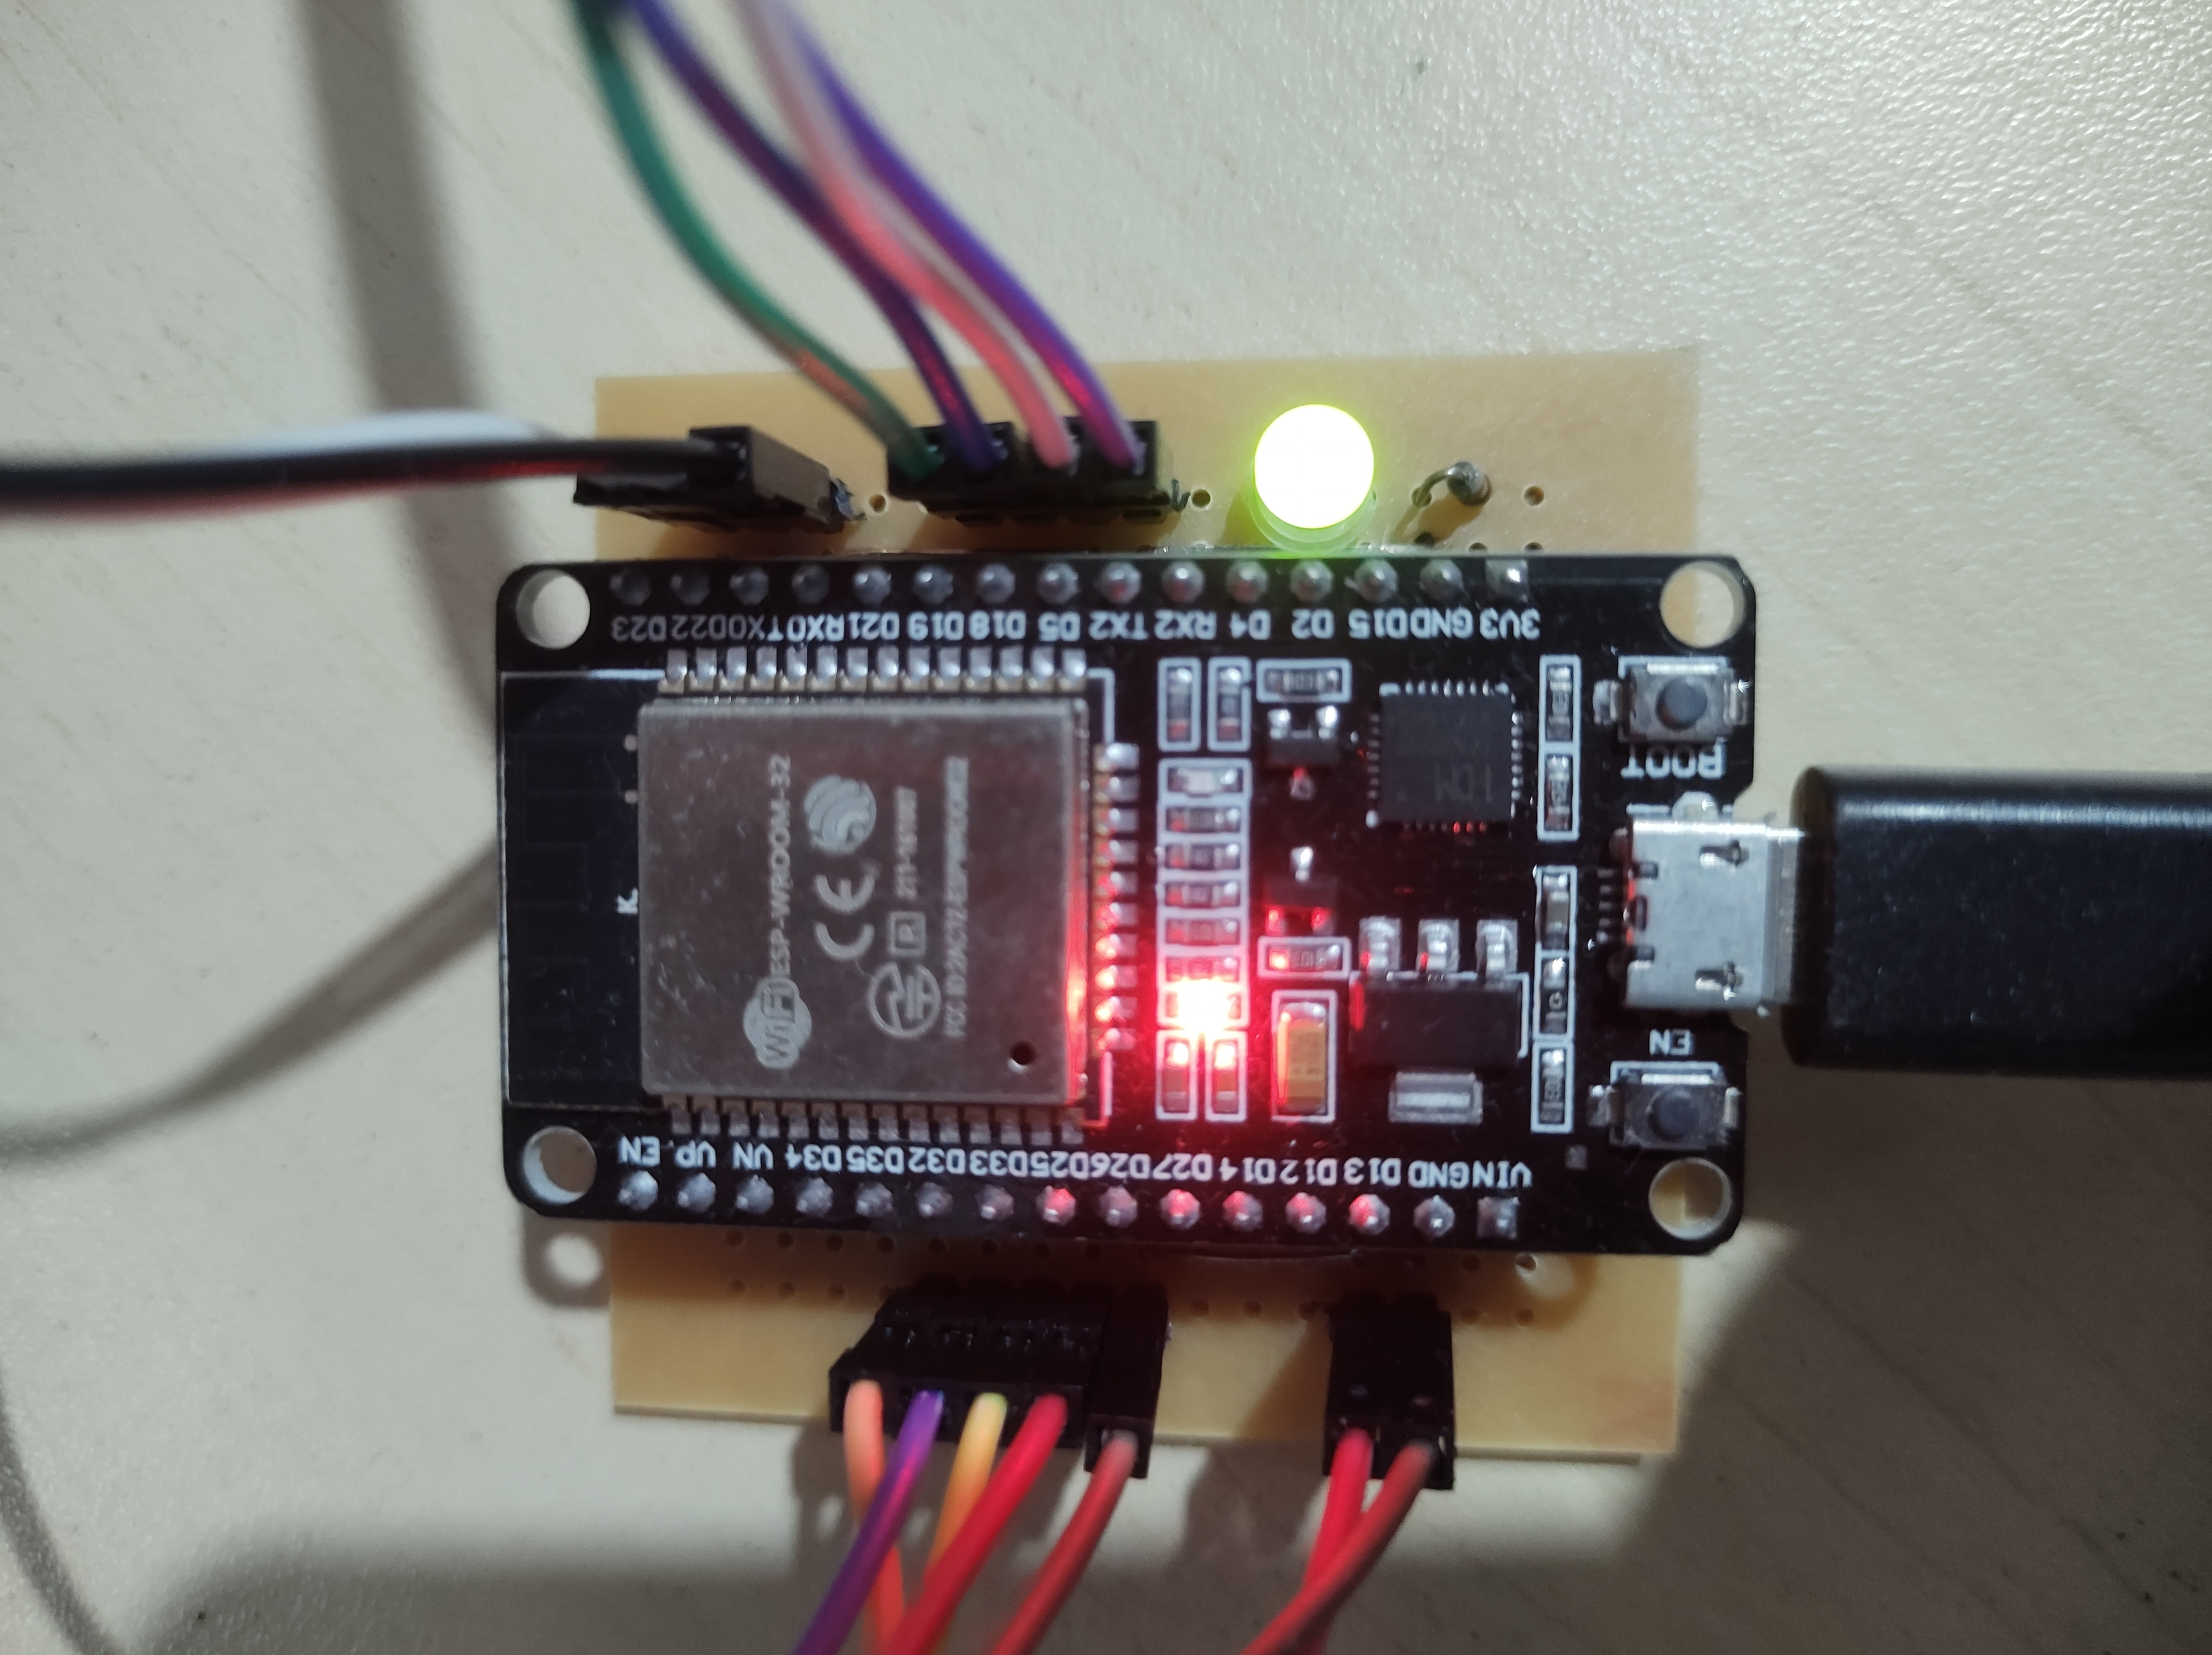
\includegraphics[scale=0.04]{Imagen 26 - Placa ESP32.jpg}
\caption[Módulo principal]{Placa del módulo principal.}
\label{fig:26}
\end{figure}

Se puede observar que se encuentra conectada con cables a los demás módulos y posee un LED rojo de encendido y un LED de 2 colores agregado para mostrar el estado de conexión a la red. Si el nodo está conectado se enciende de color verde, y si está desconectado se enciende de color rojo. Además, se utiliza un tercer LED de color azul que parpadea cuando el dispositivo envía o recibe datos por MQTT.

En el nodo de temperatura, cuando está seleccionado el modo manual y se gira el encoder, la salida se enciende o apaga dependiendo si se gira en sentido horario o antihorario. En el nodo dimer, al girar en sentido horario se aumenta un 10\% la intensidad y se disminuye un 10\% en sentido inverso. En ambos dispositivos, si el modo elegido es automático, al girar el encoder no se modifica la salida.

\subsection{Menúes y pantallas}

Cada nodo tiene la posibilidad de ser comandado desde el lugar y poder mostrar el estado y configuraciones por el display asociado. Esto es posible gracias a menúes implementados en el software que posibilitan la muestra de estos datos. En la figura \ref{fig:27} pueden verse las imágenes de las distintas pantallas del dispositivo.

\begin{figure}[h]
\centering
\includegraphics[scale=0.65]{Imagen 27 - Pantallas.jpg}
\caption[Pantallas dispositivo]{Pantallas del dispositivo.}
\label{fig:27}
\end{figure}

Para acceder al menú principal o seleccionar una opción dentro de un menú, debe apretarse el pulsador incorporado en el encoder. Para moverse por las distintas opciones se debe girar dicho encoder en sentido horario para bajar y antihorario para subir.

En la primera imagen puede verse la pantalla de saludo cuando se inicia el dispositivo. En la segunda se ve la pantalla principal en este caso del dispositivo de temperatura donde se muestra la hora, temperatura, humedad, el estado de la salida y el modo actual de funcionamiento. En la siguiente imagen se ve el primer menú donde se puede acceder a las distintas opciones. Aquí puede observarse que la opción seleccionada aparece resaltada. Luego está la imagen del estado del dispositivo, y en la que sigue la información de conexión. La imagen que sigue muestra la selección del modo de funcionamiento y la que se ve a continuación exhibe la información de configuración del modo automático. Es importante destacar que solo pueden verse los valores del modo, hora de encendido, apagado y set point, pero no pueden modificarse. Para lograr esto es necesario hacerlo desde la aplicación web. Por último se agregó una opción para actualizar la hora en caso que el dispositivo pierda la conexión.

Los menúes se implementaron mostrando en pantalla distintos textos y leyendo los valores de las variables auxiliares de posición. En el código \ref{lst:Ejemplo menu} puede verse el fragmento que muestra en pantalla las opciones y lee el valor de la variable de posición denro del mismo.

\begin{lstlisting}[caption={Código del menú principal}, label={lst:Ejemplo menu}]
void menu1 (void)
{
	ssd1306_clear_screen(&devd, false);
	pos_menu=1;
	while(level==1){
		if(inc_enc){
			pos_menu++;
			inc_enc=false;
			if (pos_menu>6)
				pos_menu=1;
		}	
		if (dec_enc){
			pos_menu--;
			dec_enc=false;
			if (pos_menu<1)
				pos_menu=6;
		}
		if(pos_menu==1){
			ssd1306_display_text(&devd, 0, "Estado          ", 16, true);
			ssd1306_display_text(&devd, 1, "Info conexion   ", 16, false);
			ssd1306_display_text(&devd, 2, "Modo            ", 16, false);
			ssd1306_display_text(&devd, 3, "Conf modo auto  ", 16, false);
			ssd1306_display_text(&devd, 4, "Actualizar hora ", 16, false);
			ssd1306_display_text(&devd, 5, "Pant. principal ", 16, false);
			if(btn_enc){
				btn_enc=false;
				level=10;
			}
		}
		if(pos_menu==2){
			ssd1306_display_text(&devd, 0, "Estado          ", 16, false);
			ssd1306_display_text(&devd, 1, "Info conexion   ", 16, true);
			ssd1306_display_text(&devd, 2, "Modo            ", 16, false);
			ssd1306_display_text(&devd, 3, "Conf modo auto  ", 16, false);
			ssd1306_display_text(&devd, 4, "Actualizar hora ", 16, false);
			ssd1306_display_text(&devd, 5, "Pant. principal ", 16, false);
			if(btn_enc){
				btn_enc=false;
				level=11;
			}
		}
		if(pos_menu==3){
			ssd1306_display_text(&devd, 0, "Estado          ", 16, false);
			ssd1306_display_text(&devd, 1, "Info conexion   ", 16, false);
			ssd1306_display_text(&devd, 2, "Modo            ", 16, true);
			ssd1306_display_text(&devd, 3, "Conf modo auto  ", 16, false);
			ssd1306_display_text(&devd, 4, "Actualizar hora ", 16, false);
			ssd1306_display_text(&devd, 5, "Pant. principal ", 16, false);	
			if(btn_enc){
				btn_enc=false;
				level=2;
			}
		}
		if(pos_menu==4){
			ssd1306_display_text(&devd, 0, "Estado          ", 16, false);
			ssd1306_display_text(&devd, 1, "Info conexion   ", 16, false);
			ssd1306_display_text(&devd, 2, "Modo            ", 16, false);
			ssd1306_display_text(&devd, 3, "Conf modo auto  ", 16, true);
			ssd1306_display_text(&devd, 4, "Actualizar hora ", 16, false);
			ssd1306_display_text(&devd, 5, "Pant. principal ", 16, false);	
			if(btn_enc){
				btn_enc=false;
				level=3;
			}
		}
		if(pos_menu==5){
			ssd1306_display_text(&devd, 0, "Estado          ", 16, false);
			ssd1306_display_text(&devd, 1, "Info conexion   ", 16, false);
			ssd1306_display_text(&devd, 2, "Modo            ", 16, false);
			ssd1306_display_text(&devd, 3, "Conf modo auto  ", 16, false);
			ssd1306_display_text(&devd, 4, "Actualizar hora ", 16, true);
			ssd1306_display_text(&devd, 5, "Pant. principal ", 16, false);
			if(btn_enc){
				btn_enc=false;
				ssd1306_display_text(&devd, 6, "Obteniendo la", 13, false);
    			ssd1306_display_text(&devd, 7, "hora...", 7, false);
				obtain_time();
				ssd1306_display_text(&devd, 7, "hora... OK", 10, false);
				vTaskDelay(pdMS_TO_TICKS(1000));
				ssd1306_display_text(&devd, 6, "               ", 15, false);
				ssd1306_display_text(&devd, 7, "               ", 15, false);
			}
		}
		if(pos_menu==6){
			ssd1306_display_text(&devd, 0, "Estado          ", 16, false);
			ssd1306_display_text(&devd, 1, "Info conexion   ", 16, false);
			ssd1306_display_text(&devd, 2, "Modo            ", 16, false);
			ssd1306_display_text(&devd, 3, "Conf modo auto  ", 16, false);
			ssd1306_display_text(&devd, 4, "Actualizar hora ", 16, false);
			ssd1306_display_text(&devd, 5, "Pant. principal ", 16, true);
			if (btn_enc){
				btn_enc=false;
				level=0;	
			}
		}
	}
	if(level==10){
			if (net_con)
				pant_conok();
			if (!net_con)
				pant_nocon();
	}
	if(level==11){
		pant_est();
	}
	if(level==2){
		menu2();
	}
	if(level==3){
		menu3();
	}
	if(level==0){
		pant_main();
	}
}
\end{lstlisting}

\subsection{Modelo de programación}

Los nodos fueron programados de forma modularizada, teniendo un código principal en el archivo \textit{main.c} reducido con funciones definidas. En el código \ref{lst:main.c} puede verse el fragmento de código del módulo principal del software embebido del dispositivo de temperatura.

\begin{lstlisting}[caption={Código de \textit{main.c}}, label={lst:main.c}]
void app_main(void)
{
    
	ESP_ERROR_CHECK(nvs_flash_init());
	ESP_ERROR_CHECK(esp_netif_init());

	_queue = xQueueCreate(QUEUE_LENGTH, sizeof(rotary_encoder_event_t));

	config_dis ();
	pant_bienv ();
	config_led();
	pant_inicio ();
	wifi_init_sta();
    if(net_con)
		mqtt_app_start();
	
	ESP_ERROR_CHECK(rotary_encoder_init(_queue));
	ESP_ERROR_CHECK(rotary_encoder_add(&control));
	
	btn_enc=false;
	ssd1306_clear_screen(&devd, false);
	xTaskCreate(get_temp, "get_temp", 4096*8, NULL, 3, NULL);
	xTaskCreate(read_enc, "read_enc", 4096*2, NULL, 4, NULL);
	power_on_device();
}
\end{lstlisting}

Aquí se inicializa el microcontrolador, el encoder y el display. Luego se conecta a la red y si lo consigue, inicializa el módulo de comunicación MQTT. Por último, se crean las tareas más importantes del sistema, la de leer la temperatura y comparar los valores del encoder para leer el sentido de giro y pulsación del botón.

En el nodo de temperatura se lee cada 5 segundos y se incrementa un contador en una unidad. Cada vez que es leída se refresca el valor en pantalla. Si dicho contador llega a un valor de 60 (lo que equivale a 5 minutos) se envían los valores al servidor. Caso contrario sigue el desarrollo del programa. En el código \ref{lst:temp.c} se puede ver el fragmento de ejecución de tareas al leerse dicho valor.

\begin{lstlisting}[caption={Código de lectura de temperatura}, label={lst:temp.c}]
void get_temp(void *pvParameter)
{
    while(1) {
        set_times();
        if (dht_read_data(sensor_type, dht_gpio, &humidity, &temperature) == ESP_OK) {
            ESP_LOGI(TAG,"Humidity: %d%% Temperature: %dC\n", humidity/10, temperature/10);
            if (!time_sinc_ok)
                obtain_time();
            time_t now = time(NULL);
            now-=3*3600;
            timeinfo = localtime(&now);
            strftime(pant_time, sizeof(pant_time), "%H:%M %d-%m-%Y", timeinfo);
            now = time(NULL);
            timeinfo = localtime(&now);
            strftime(formatted_time, sizeof(formatted_time), "%Y-%m-%d %H:%M:%S", &timeinfo);
            sprintf(hum_char, "%d", humidity/10);
			sprintf(temp_char, "%d", temperature/10);
            if(level==0)
                pant_main();
            esp_wifi_sta_get_ap_info(&ap_info);
            net_con = (ap_info.authmode != WIFI_AUTH_OPEN);
            if(cont_mqtt==60)
                {
                cont_mqtt=0;
                if (net_con==false)
                    esp_wifi_connect();
                if(mqtt_state)    
                    mqtt_send_info();
                }
            cont_mqtt++;
            if(modo==1){
                if(time_func && ((temperature/10)<=(set_point-hist))){
                    out_temp=true;
                    gpio_set_level(CONTROL, 1);
                }
                if(time_func && ((temperature/10)>=(set_point+hist))){
                    out_temp=false;
                    gpio_set_level(CONTROL, 0);
                }
                if(!time_func){
                    out_temp=false;
                    gpio_set_level(CONTROL, 0);
                }
            }
            vTaskDelay(pdMS_TO_TICKS(1000*refresh));
        } else {
            if (cont_temp > 5){
                ESP_LOGE(TAG,"Could not read data from sensor\n");
			    pant_no_sensor();
                }
            cont_temp++;
            xTaskDelayUntil(&xLastWakeTime, pdMS_TO_TICKS(100));
        }
    }
   vTaskDelete(NULL);
}
\end{lstlisting}

En el nodo de dimer el funcionamiento es el mismo y el código muy similar, con la diferencia que se envía el valor de la salida ya que no posee sensores de entrada que estén leyendo parámetros.

\subsection{Especificaciones de los sensores}

A continuación se listan sensores utilizados con sus principales características:

\begin{itemize}
	\item DHT22: sensor de temperatura y humedad relativa ambiente \citep{31}.
	\begin{itemize}
		\item Rango de temperatura: -40 a 80 grados Celsius.
		\item Resolución: 0,1 grado Celsius.
		\item Comunicación: serie, bus de 1 hilo, 40 bits por trama.
	\end{itemize}
	\item KY-040: encoder rotativo con interruptor. 20 pulsos por vuelta \citep{32}.
\end{itemize}

En la figura \ref{fig:28} se muestra la imagen del encoder a la izquierda y del sensor de temperatura a la derecha con sus correspondientes esquemas de conexión.

\begin{figure}[h]
\centering
\includegraphics[scale=1.4]{Imagen 28 - Sensores.jpg}
\caption[Sensores]{Sensores utilizados.}
\label{fig:28}
\end{figure}

\subsection{Especificaciones de los actuadores}

\begin{itemize}
\item SSD1306: display OLED 1,2 pulgadas.
	\begin{itemize}
		\item Resolución: 128x64 píxeles.
		\item Interfaz: I2C.
	\end{itemize}
	\item Control de potencia para 220 V: módulo con aislación y salida de triac. Se utilizó un triac BT137 \citep{33} y un optoacoplador MOC3041 \citep{34}.
	\begin{itemize}
		\item Tipo: encendido - apagado (on - off).
		\item Carga máxima: 8 A.
		\item Tipo de aislación: optoacoplador.
		\item Tensión máxima de aislación: 7500 V AC pico, 1 segundo de duración.
	\end{itemize}
	\item Control de intensidad de luz: módulo de control para iluminación LED de corriente continua implementado con modulación por ancho de pulso (PWM). Se utilizó un transistor BC337 \citep{35}.
	\begin{itemize}
		\item Tipo: PWM y encendido - apagado (on - off).
		\item Carga máxima: 800 mA CC.
		\item Tensión de alimentación: 5 a 24 V CC.
	\end{itemize}
\end{itemize}

En la figura \ref{fig:29} se muestra la imagen del circuito de potencia montado en una caja estanca a la izquierda y del control por ancho de pulso a la derecha con sus correspondientes esquemas de conexión.

\begin{figure}[h]
\centering
\includegraphics[scale=1.4]{Imagen 29 - Actuadores.jpg}
\caption[Actuadores]{Actuadores utilizados.}
\label{fig:29}
\end{figure}

\section{Comunicación del sistema}

